\chapter{Expression des besoins}
\clearpage
\section{introduction}
Ce projet vise à créer une marketplace dédiée à la restauration, où chaque utilisateur aura la possibilité de lancer et de gérer son propre restaurant en ligne. Grâce à une interface intuitive, il pourra personnaliser son espace, gérer son menu, suivre les commandes en temps réel et administrer son personnel selon ses besoins.  

L’objectif est d’offrir une solution flexible et évolutive qui permettra aux restaurateurs, qu’ils soient indépendants ou en réseau, d’optimiser leur gestion et d’atteindre une clientèle plus large. Cette plateforme mettra également à disposition des outils de suivi des performances, des options de paiement sécurisées et des fonctionnalités facilitant l’interaction avec les clients.  

En intégrant des fonctionnalités modernes et une expérience utilisateur fluide, cette marketplace ambitionne de révolutionner la manière dont les restaurants gèrent leurs activités en ligne.  


\subsection{Spécifications techniques}

\subsubsection{Langages et Technologies}
\begin{itemize}
    \item \textbf{Framework :} Laravel (passport) pour une gestion efficace de la logique serveur et du backend (developpement d'api).
    \item \textbf{Base de données :} MySQL ou PostgreSQL pour la gestion des données avec Eloquent ORM.
    \item \textbf{Frontend :} React js pour une interface utilisateur dynamique et fluide.

\end{itemize}


\subsubsection{Sécurité}
\begin{itemize}
    \item Chiffrement des données sensibles.
    \item Gestion des accès par rôles.
\end{itemize}

\subsubsection{Hébergement}
\begin{itemize}
    \item Déploiement sur les serveurs internes de Sirius Digital.
\end{itemize}
\subsection{Exigences non fonctionnelles}



\subsubsection{Utilisabilité}
\begin{itemize}
    \item L'interface utilisateur doit être intuitive et facile à utiliser, avec une courbe d'apprentissage minimale.
    \item Une documentation utilisateur complète doit être fournie, incluant des guides et des tutoriels.
\end{itemize}

\subsubsection{Compatibilité}
\begin{itemize}
    \item \textbf{Navigateurs :} Le logiciel doit être compatible avec les dernières versions de Chrome, Firefox, Safari, et Edge.
    \item \textbf{Mobile :} L'application web doit être responsive et accessible depuis les navigateurs mobiles.
\end{itemize}

\subsubsection{Scalabilité}
Le logiciel doit pouvoir gérer un nombre croissant d'utilisateurs et de données sans dégradation des performances.


\subsubsection{Nom du logicièl}
Le logiciel portera donc le nom S


\section{Définition des acteurs système}
Le logiciel est destiné à tous les utilisateurs souhaitant créer et gérer leur propre restaurant.
\begin{itemize}
    \item Client
    \item Serveur 
    \item Caissier
    \item ChefSection
    \item DG 
\end{itemize}
\subsection{Client}
L'utilisateur \textbf{Client} est simplement un utilisateur quelconque qui peut utiliser le logiciel pour commander un plat.
De même après s'être inscrit, a aussi le choix de créer et gérer son propre restaurent.
\subsection{Serveur}
Le \textbf{Serveur} est un personnel appartenant à un restaurent donné qui inter-agit avec le système pour passer des commandes en interne pour les client sur place.

\subsection{Caissier }
Le \textbf{Casier} est un personnel appartenant à un restaurent donné qui enregistrer les factures et gères beaucoup d'autres choses.

\subsection{ChefSection}
Le \textbf{DG} est un personnel appartenant à un restaurent donné, il est en quelque sorte le sous directeur du restaurent auquel il appartient. De ce fait il à beaucoup de responsabilité.

\subsection{DG}
Le \textbf{DG} est le propriétaire du restaurent, de ce fait il a le contrôle absolu du système de gestion du restaurent à travers l'application.

\section{D\'efinition des cas d'utilisation}

Un diagramme de cas d'utilisation est une représentation graphique des interactions entre les acteurs d'un système et ses fonctionnalités. Il permet d'identifier et de structurer les besoins fonctionnels du logiciel en décrivant les actions réalisées par chaque acteur. Ce type de diagramme est particulièrement utile pour comprendre les interactions des utilisateurs avec le système et pour définir clairement les responsabilités de chaque acteur.

Dans ce contexte, nous définissons les cas d'utilisation pour chaque fonctionnalités énoncés précédemment.
\subsection{Listes des cas d'utilisation}
\subsubsection{Description de chaque fonctionalité}
Cette application en son sein regroupe beaucoup de fonctionnalités telles que :
\subsubsection{Gestion de restaurent}
\begin{itemize}
    \item \textbf{Créer un restaurent :} Une fois sur l'application tout utilisateur doit visiter le guide d'utilisation de l'application et, créer autant de restaurent comme il le souhaite et gérer son personnel.
    \item \textbf{Créer une section :} Ici l'utilisateur pour passer en mode DG du restaurent doit payer son abonnement et en suite, il pourra donc : Créer des section pour chaque restaurent, gérer son personnel en fonction de leurs rôles. 
    \item \textbf{Gestion des rôles :} En tant que DG de son restaurent, lui seul a le droit de gérer les rôles et permissions de ses employés a sa guise.
\end{itemize}

\subsubsection{Gestion Séparée}
\begin{itemize}
    \item \textbf{Rôle ChefSection :} On es conscient que pour un restaurent pratiquement impossible de gérer sa seule. Bien que toutes les actions que font les autres employés, le DG est au courant, il se doit de partager les rôles. Ainsi le chefSection gère les fonctionnalités suivantes : 
    \subsubsection{Gestion Catégorie}
    \subsubsection{Gestion Promotion}
    \subsubsection{Gestion Plat}
    \subsubsection{Gestion Réservation}
    \subsubsection{Gestion des Tables}
    \subsubsection{Gestion des Commandes}
    \subsubsection{Gestion des Événement}
    
    \item \textbf{Rôle Serveur : } Le serveur agit sur le système pour passer des commandes pour des clients en internes
\end{itemize}


\section{Illustration des fonctionnalités à travers les diagrammes de cas d'utilisation}

\subsubsection{Diagramme de cas d'utilisation par acteur du système}
\begin{figure}[H]
    \centering
    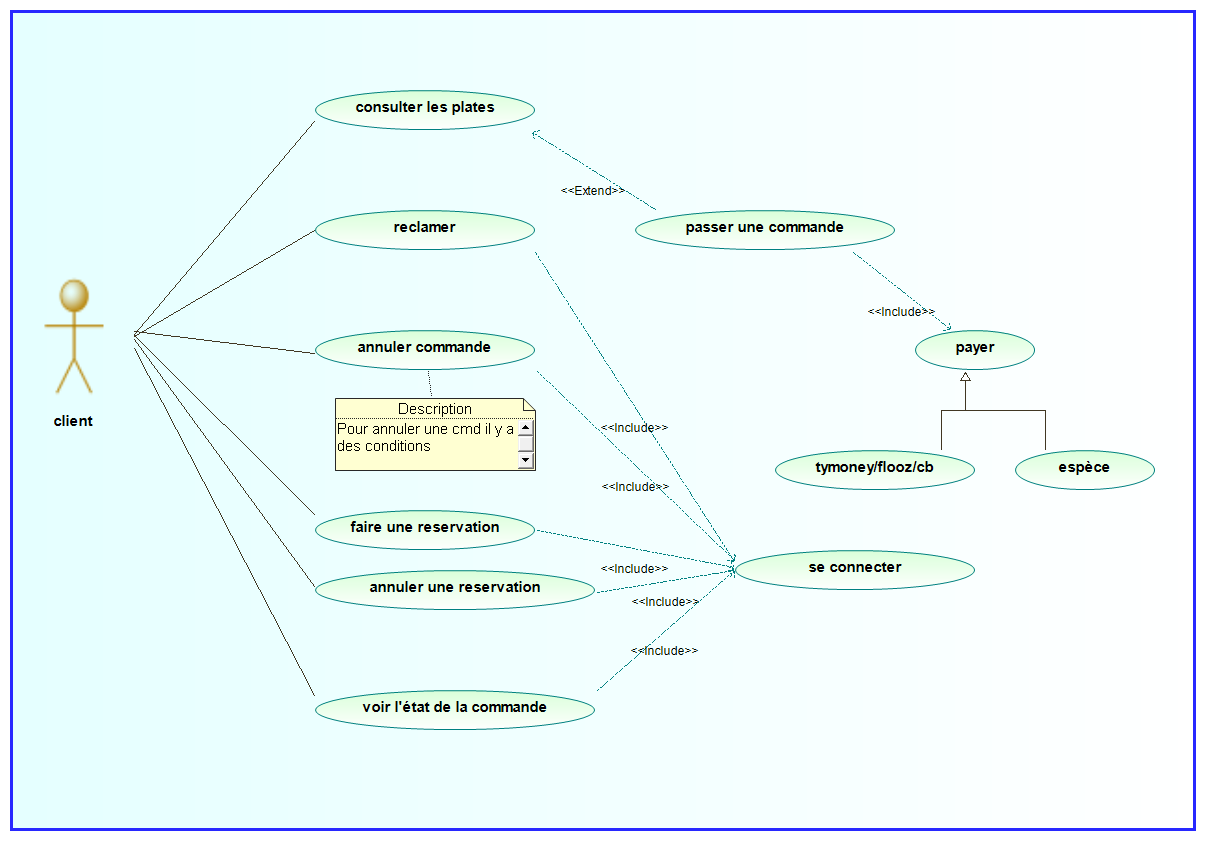
\includegraphics[width=0.8\textwidth]{images/diagrammes/use-cases/client.png}
    \caption{Diagramme de cas d'utilisation Gestion des Congés et Absences}
    \label{fig:use_case_gestion_conges}

\end{figure}


\begin{figure}[H]
    \centering
    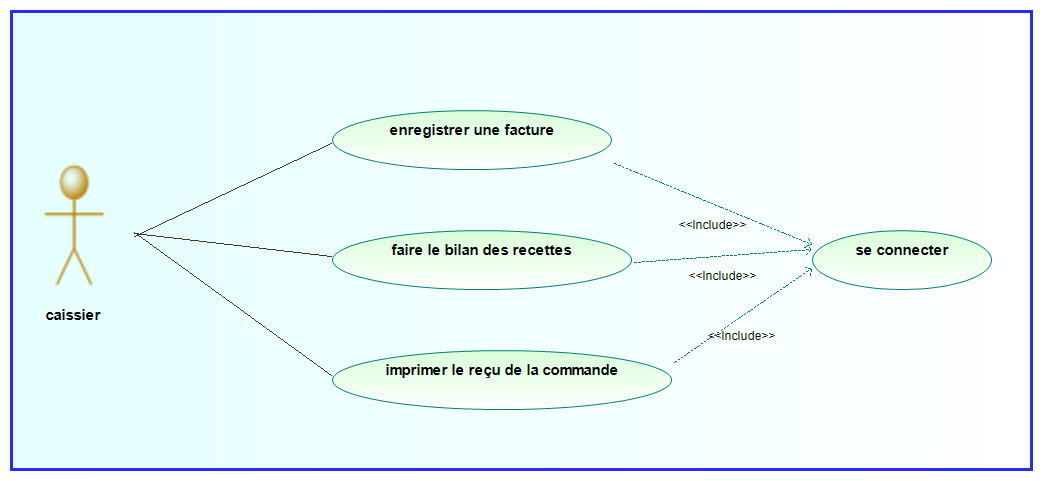
\includegraphics[width=0.8\textwidth]{images/diagrammes/use-cases/caissier.png}
    \caption{Diagramme de cas d'utilisation Gestion des Congés et Absences}
    \label{fig:use_case_gestion_conges}

\end{figure}


\begin{figure}[H]
    \centering
    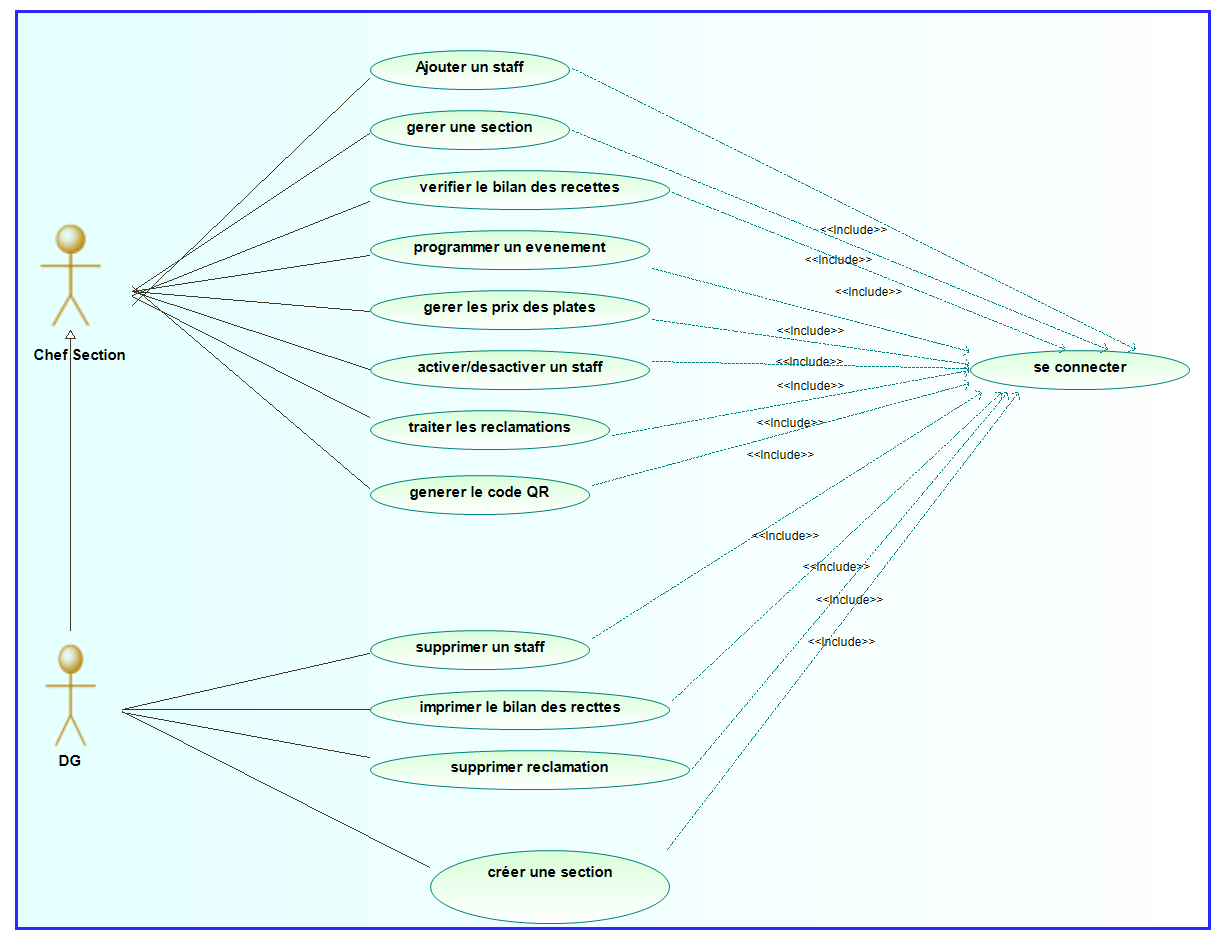
\includegraphics[width=0.8\textwidth]{images/diagrammes/use-cases/DG.png}
    \caption{Diagramme de cas d'utilisation Gestion des Congés et Absences}
    \label{fig:use_case_gestion_conges}

\end{figure}



\section{En résumé}
Le cahier des charges définit les fonctionnalités et les exigences techniques de ce logiciel faisant office d'un marché de restauration en ligne pour tous.
\clearpage
